\subsection{Mecanismos de Atención} \label{section:att}

Una de las arquitecturas comunes vistas previamente es la mostrada en la figura \ref{fig:rnn_cfgc} cuya información
procesada es resumida en una sola salida. Este tipo de red es usada como parte de las soluciones en
tareas de reconocimiento de voz (\textit{Speech Recognition}), traducción de lenguaje
(\textit{Machine Translation}) o asistencia en respuestas automáticas (\textit{Question Answering}), entre
otros,
típicamente bajo modelos Secuencia a Secuencia (\textit{Sequence to Sequence, Seq2Seq})
\cite{DBLP:journals/corr/ChoMGBSB14}. Los modelos
\textit{Seq2Seq} están formados por dos redes neuronales como la mostrada en \ref{fig:seq2seq}. La
primera se comporta como un \textit{codificador} al resumir la entrada y producir un vector de salida
de tamaño fijo llamado \textit{vector de contexto}. La segunda red se comporta como un
\textit{decodificador}, este es inicializado y condicionado con el
\textit{vector de contexto} para obtener una transformación de la entrada no necesariamente del
mismo tamaño de secuencia, debido a que en tareas como traducir una oración de un lenguaje a otro
donde la traducción no siempre contiene las misma cantidad de palabras usadas en el idioma original.

\begin{figure}[ht!]
    \centering
    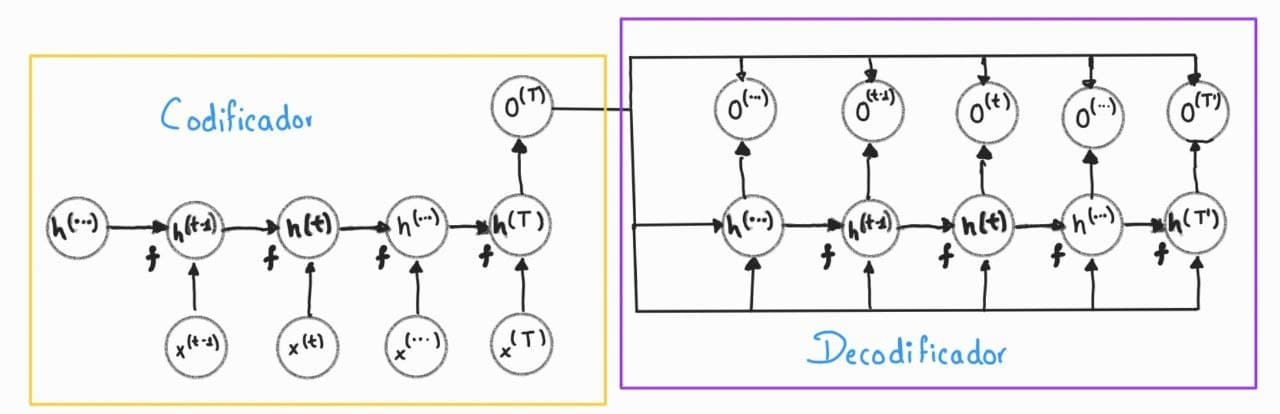
\includegraphics[width=1.0 \textwidth]{Chapters/2. Transformer/Figures/rnn/seq2seq.jpg}
    \caption{Descripción.}
    \label{fig:seq2seq}
\end{figure}

Por ejemplo, en tareas de \textit{Machine Translation} el \textit{codificador} esta formado por una
\textit{RNN} Bidireccional que lee y procesa un conjunto de
vectores $X = (x^{(1)}, x^{(2)}, \dots, x^{(T_x)})$ para obtener un vector de contexto $C$. La forma
más común es como en \ref{eq:s2s_simple}:

\begin{equation}
    \begin{split}
        h^{(t)} = f_{bi}(x^{(t)}, h^{(t-1)}; \theta_{f}, \theta_{b}) \\
        C = q({h^{(1)}, h^{(2)}, \dots, h^{(T)}})
    \end{split}
    \label{eq:s2s_simple}
\end{equation}

Recordemos que $h^{(t)}$ es el estado oculto generado por la concatenación de los dos estados ocultos
generados por la \textit{RNN Bidireccional}, $f_{bi}$ y $q$ son funciones no lineales, ya sea,
una \textit{LSTM} para $f_{bi}$ y $q({h^{(1)}, h^{(2)}, \dots, h^{(T)}}) = h^{(T)}$, equivalente a
tomar solo el ultimo estado oculto como vector de contexto $C$. El \textit{decodificador} es entrenado
para predecir la siguiente palabra $y^{(t')}$ dado el vector de contexto $C$ y todas las palabras
previas predichas. En otras palabras, el decodificador define la probabilidad conjunta modelada por una
\textit{RNN}:

\begin{equation}
    p(Y) = \prod_{t=1}^{T_y} p(y^{(t)} | \{y^{(1)}, \dots , y^{(t-1)}\}, C)
\end{equation}
\begin{equation}
    p(y^{(t)} | \{y^{(1)}, \dots , y^{(t-1)}\}, C) = g(y^{(t-1)}, s^{(t)}, C; \theta_g)
\end{equation}

donde $g$ es una función no lineal que emite la probabilidad de $y^{(t)}$ y $s^{(t)}$ es el estado oculto
del \textit{decodificador} \ref{eq:sqs_s}.

\begin{equation}
    s^{(t)} = f(s^{(t)}, y^{(t-1)}, C; \theta_s)
    \label{eq:sqs_s}
\end{equation}


Sin embargo, cuando las secuencias son bastante largas el \textit{vector de contexto} emitido por el
\textit{codificador} no es lo suficientemente grande como para resumir correctamente la secuencia y
por tanto, la información inicial de la entrada es olvidada, teniendo escasa presencia en estados
ocultos más lejanos. En 2015 \citeauthor*{bahdanau2016neural} observaron estos efectos y
propusieron una forma de minimizarlos, los \textbf{Mecanismos de Atención}.

La función principal de los \textbf{Mecanismos de Atención} es permitir que el \textit{decodificador}
pueda acceder al historial completo de los estados ocultos del \textit{codificador}, así, ahora podrá
contar con un mecanismo
para selectivamente centrarse en las distintas partes de la secuencia que tienen mayor influencia sobre
una la salida esperada a cierto tiempo.

Por tanto, las palabras predichas no son calculadas por un único \textit{vector de contexto} generado por
el \textit{codificador}, sino que para cada objetivo $y^{(t)}$ se calcula un nuevo \textit{vector de contexto} $c^{(t)}$:

\begin{equation}
    p(y^{(t)} | \{y^{(1)}, \dots , y^{(t-1)}\}, c^{(t)}) = g(y^{(t-1)}, s^{(t)}, c^{(t)}; \theta_g)
\end{equation}

\begin{equation}
    s^{(t)} = f(s^{(t)}, y^{(t-1)}, c^{(t)}; \theta_s)
\end{equation}

Dado que cada estado oculto $h^{(t)}$ contiene mucho mejor la información que se encuentran alrededor
del t-ésimo término, se puede generar cada vector de contexto como una suma pesada de sobre los
estados ocultos del \textit{codificador}. Estos pesos nos ayudan a determinar que tan importante es la
información codificada por cada estado oculto y al momento de obtener la salida del t-ésimo valor
\quotes{prestar atención} a aquellos que son más relevantes para esta predicción:

\begin{equation}
    c^{(t)} = \sum_{i=1}^{T_x} \alpha_{t,i} h^{(i)}
\end{equation}

aquí cada peso $\alpha_{t,i}$ indica que tan bien se \quotes{alinean} los términos $y^{(t)}$ y $x^{(i)}$,
y son calculados por una \textit{función de alineamiento} que denota que tan importante es el estado
oculto del \textit{codificador} $h^{(t)}$ para el estado oculto del decodificador $s^{(i)}$.

\begin{equation}
    \alpha_{t,i} = align(y^{(t)}, x^{(i)}) = \frac{\exp(score(s^{(t-1)}, h^{(i)}))}{\sum_{k=1}^{T_x} \exp(score(s^{(t-1)}, h^{(k)}))}
    \label{eq:b_align}
\end{equation}

\textit{Bahdanau} propone aprender esta alineación usando una \textit{Red feed-forward} con una sola
capa oculta y la función $\tanh$ como activación:

\begin{equation}
    score(s^{(t)}, h^{(i)}) = v^\top_a \tanh(W_a[s^{(t)};h^{(i)}])
    \label{eq:concat}
\end{equation}

con $v_a$ y $W_a$ como matrices de pesos a aprender durante el entrenamiento, $[s^{(t)};h^{(i)}]$
representa una concatenación de los estados ocultos del \textit{codificador} y decodificador. En la figura
\ref{fig:att} podemos ver gráficamente el modelo usado por \textit{Bahdanau}.

\begin{figure}[ht!]
    \centering
    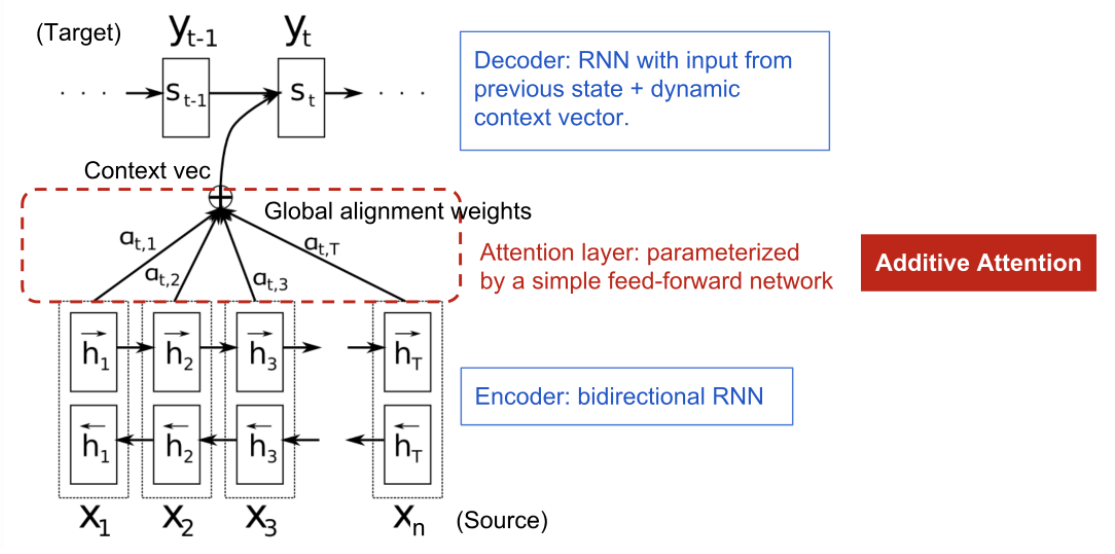
\includegraphics[width=0.8 \textwidth]{Chapters/2. Transformer/Figures/rnn/attention.png}
    \caption{Modelo seq2seq propuesto por \citeauthor*{bahdanau2016neural} con \textit{Additive/Concat Attention}}
    \label{fig:att}
\end{figure}

Los modelos de atención pueden ser vistos de manera más general como un mapeo de una secuencia de
llaves $k$ hacia una distribución de atención $\alpha$ de acuerdo a una consulta $q$ aplicándose a un
conjunto de valores $V$ para selectivamente propagar la información contenida en $V$.
Si bien, los términos de consulta, llaves y valores (query, keys, values)
son en ámbitos de los \textit{Sistemas de Recuperación de Información} su relación en términos de
la atención aplicada por Bahdanau es muy similar; las llaves son los estados ocultos del \textit{codificador}
y la consulta es el estado oculto del decodificador en cuestión, en este caso el mapeo de entre llaves
y valores es la misma:

\begin{equation}
    A(q, K, V) = \sum_i p(a(K-i, q)) * v_i
    \label{eq:att_general}
\end{equation}

En la ecuación \ref{eq:att_general}, $p$ es una función de distribución que mapea los puntajes de la
función de alineación $a$ a pesos de atención. Comúnmente se usan las funciones \textit{softmax} o
\textit{logistic sigmoid} puesto que nos aseguran que los pesos de atención producidos estarán dentro
del rango $[0,1]$ y la suma de ellos es igual a $1$, por lo que los pesos pueden ser interpretados como
una probabilidad que indica que tan relevante es cierto elemento. Algunas variaciones en donde se
consideran solo los términos relevantes como \textit{sparsemax} \citeauthor*{DBLP:journals/corr/MartinsA16}
o \textit{sparse entmax} \citeauthor*{DBLP:journals/corr/abs-2006-07214} permiten trabajar y enfocarse
en solo algunas relaciones de alineamiento. \citeauthor*{NEURIPS2019_16fc18d7} proponen una función de
distribución de pesos $M = \tanh(E) \odot sigmoid(N)$ con $E$ como una matrix en donde cada entrada
representa la similaridad entre estados ocultos y $N$ una medida negativa (disimilaridad), por lo que
podemos usar
$sigmoid(N)$ como información para \quotes{de-atender} los alineamientos de $E$.

Las funciones de alineamiento se encargan de comparar y extraer la relación entre las representaciones de las llaves (keys) y
consultas (queries), por ejemplo usando el producto punto y el coseno como función de similaridad.
Bahdanau calcula esta relación a través de una red neuronal \ref{eq:b_align}, lo que evita asumir
que ambas representaciones están en el mismo espacio, como lo hace las funciones de alineación
como el producto punto o la similaridad coseno. La tabla \ref{Tab:att} muestra una
recopilación de funciones de alineamiento.


\begin{table}[ht!]
\begin{center}
\begin{tabular}{@{}lll@{}}
\toprule
\textbf{Nombre} & \textbf{Función de Alineación} & \textbf{Cita} \\
\midrule
Similarity / Content-Base & $a(k_i, q) = sim(k_i, q)$ & \citeauthor*{DBLP:journals/corr/GravesWD14} \\ \\
Dot Product\textsuperscript{1} & $a(k_i, q) = q^\top k_i$ & \citeauthor*{DBLP:journals/corr/LuongPM15} \\ \\
Scaled Dot Product & $a(k_i, q) = \frac{q^\top k_i}{\sqrt{d_k}}$ & \citeauthor*{DBLP:journals/corr/VaswaniSPUJGKP17} \\ \\
General & $a(k_i, q) = q^\top W k_i$ & \citeauthor*{DBLP:journals/corr/LuongPM15} \\ \\
Biased General & $a(k_i, q) = k_i (Wq + b )$ & \citeauthor*{DBLP:journals/corr/SordoniBB16} \\ \\
Activated General & $a(k_i, q) = act(q^\top W k_i + b)$ & \citeauthor*{DBLP:journals/corr/abs-1709-00893} \\ \\
Generalized Kernel & $a(k_i, q) = \phi(q)^\top \phi(k_i)$ & \citeauthor*{DBLP:journals/corr/abs-2009-14794} \\ \\
Additive\textbackslash Concat \textsuperscript{2} & $a(k_i, q) = v^\top act(W[q;k_i]+ b)$ & \citeauthor*{bahdanau2016neural}, \citeauthor*{DBLP:journals/corr/LuongPM15} \\ \\
Deep & $a(k_i, q) = v^\top E^{(L-1)} + b^L$ & \citeauthor*{Pavlopoulos} \\
    & $E(l) = act(W_l E^{(l-1)} + b^l)$ &  \\
    & $E(1) = act(W_0k_i + W_1q + b^l)$ &  \\ \\
Location-based & $a(k_i, q) = act(W q)$ & \citeauthor*{DBLP:journals/corr/LuongPM15} \\ \\
Feature-based & $a(k_i, q) = v^\top act(W_0 \phi(K) + W_1 \phi(K) + b)$ & \citeauthor*{DBLP:journals/corr/abs-1810-10126} \\
\bottomrule
\end{tabular}
\end{center}
\caption{Distintos tipos de funciones de alineación. (Tabla basada en \cite{DBLP:journals/corr/abs-1904-02874} \cite{weng2018attention}). \\
$a(k_i, q)$ representa la función de alineación entre $k_i$ y $q$ y $act$ es una función de activación. \\
$sim$ es una función de similaridad, \citeauthor*{DBLP:journals/corr/GravesWD14} propone la función coseno.\\
Los parámetros $v, W, W_1, W_2$ son parámetros aprendidos por la red neuronal.\\
\textsuperscript{1} El factor de escala $\frac{1}{\sqrt{d_k}}$ ayuda a estabilizar cuando el
gradiente es muy pequeño. $d_k$ es el tamaño de la cabeza de atención.\\
\textsuperscript{2} La función de activación propuesta por \citeauthor*{bahdanau2016neural} es la función $tanh$ como se ve en \ref{eq:concat} \\
\label{Tab:att}}
\end{table}

De acuerdo a como es aplicado los distintos tipos de atención \citeauthor*{DBLP:journals/corr/abs-1904-02874}
los dividen en 4 grandes grupos; por número de secuencias, por nivel de abstracción, por número de
posiciones y por número de representaciones. Estos grupos no son mutualmente excluyentes por tanto
una aplicación de atención puede pertenecer a más de una.

En la categoría \textit{por número de secuencias} se identifican 3 tipos, el primero de ellos,
\textbf{Distintivos} (\textit{Distinctive}) es cuando la clave (key) y valor (value) pertenecen a
distintas secuencias de entrada y salida respectivamente, como es el caso del modelo propuesto por
\citeauthor*{bahdanau2016neural}. El segundo tipo, \textbf{Co-Atención} (\textit{co-attention}) utiliza
distintos secuencias al mismo tiempo para conocer los pesos de atención entre estas entradas. Por ejemplo,
en tareas en donde se necesita trabajar con datos multi-modales como procesar imágenes y texto
simultáneamente. En tareas como \textit{Visual Question Answering}
se puede aplicar un mecanismo de atención conjunto tanto para las imágenes y el texto para identificar
las regiones de la imagen y los palabras del texto que son más relevantes. El
tercer tipo es \textbf{auto-atención} (\textit{Self Attention}), fue propuesto por \citeauthor*{yang2016hierarchical} y es uno
de los puntos claves para los modelos \textit{Transformers} \cite{DBLP:journals/corr/VaswaniSPUJGKP17}.
Es comúnmente usada en tareas que solo requieren una salida resumen y no una secuencia como \textit{
Clasificación de texto}. La clave (key) y valor (value) pasan a ser las mismas y la atención es
calculada sobre los mismos elementos pertenecientes a la secuencia de entrada, buscando
así, encontrar las relaciones entre las palabras de la misma oración.

La segunda Categoría agrupa la atención por el nivel de abstracción en la que es aplicada, a un
\textbf{solo nivel} o en \textbf{múltiples niveles}. La información a procesar muchas veces puede ser
representada en distintos niveles de abstracción, es decir, en texto, podemos separar los datos a
nivel de letras, n-gramas, palabras, oraciones, párrafos, etc., por tanto, es posible atender
de manera jerárquica a las palabras que forman una oración para posteriormente prestar atención a
las oraciones que conformar un texto más largo. \citeauthor*{yang2016hierarchical} utiliza este procedimiento
para generar un vector de características usado posteriormente en un etapa de clasificación.

En la tercer categoría la atención es realizada en diversas partes de la secuencia; la suma pesada sobre
todos los puntajes de las entradas usada por \citeauthor*{bahdanau2016neural} se le denomina \textbf{
Atención suave} (\textit{Soft-Attention}). Una alternativa es la \textbf{Atención dura}
(\textit{Hard-Attention}) \cite{DBLP:journals/corr/XuBKCCSZB15} que calcula la atención no sobre todas
los puntajes de alineamiento sino en una parte de estos, para ello se usa una distribución multinoulli
parametrizada por los pesos de la atención. A pesar de que es más eficiente que la
\textit{atención suave} resulta difícil de entrenar al no ser completamente diferenciable. Otra opción
a la \textit{atención dura} es la \textbf{Atención Local} (\textit{Local Attention}) cuya idea es aplicar
atención sobre una ventana elegida ya sea centrada con respecto a la tiempo actual (alineamiento monotónico)
o predicha por una función (alineamiento predictivo). La \textit{atención local} fue propuesta por
\citeauthor*{DBLP:journals/corr/LuongPM15} así como la \textit{Atención Global} la cual es similar a la
\textit{atención suave}.

La última categoría divide los modelos de atención por las formas de representación de las entradas
sobre las que la atención es aplicada. Distintos modelos pueden beneficiarse de procesar los datos
creando vectores de características distintos, cada uno de ellos deriva de algún tipo de representación
de la entrada. por tanto, es posible atendera a diferentes representaciones y formar un vector
final usando una combinación pesada de estos a través de dichos pesos de atención.
\citeauthor*{DBLP:journals/corr/abs-1904-02874} llama a este tipo de modelos de atención como
\textbf{multi-representational AM}. En la segunda categoría,
\textbf{milti-dimensional attention}, la atención no es aplicada sobre los diversas vectores de
características sino a un nivel más interno,
sobre sus dimensiones. Pesando cada característica de un vector de características permite seleccionar
aquellas que mejor lo describen para un contexto dado. EN \textit{NLP}, resulta bastante útil cuando se trata
con \textit{polisemia}, en donde una palabra o frase puede tener más de un significado.
